\documentclass[12pt]{article}

\usepackage{fullpage}
\usepackage{multicol,multirow}
\usepackage{tabularx}
\usepackage{ulem}
\usepackage[utf8]{inputenc}
\usepackage[russian]{babel}
\usepackage{amsmath}
\usepackage{amssymb}
\usepackage{graphicx}
\usepackage{hyperref}


\usepackage{titlesec}

\titleformat{\section}
  {\normalfont\Large\bfseries}{\thesection.}{0.3em}{}

\titleformat{\subsection}
  {\normalfont\large\bfseries}{\thesubsection.}{0.3em}{}

\titlespacing{\section}{0pt}{*2}{*2}
\titlespacing{\subsection}{0pt}{*1}{*1}
\titlespacing{\subsubsection}{0pt}{*0}{*0}
\usepackage{listings}
\lstloadlanguages{Lisp}
\lstset{extendedchars=false,
	breaklines=true,
	breakatwhitespace=true,
	keepspaces = true,
	tabsize=2
}
\begin{document}


\section*{Отчет по лабораторной работе №\,3
по курсу \guillemotleft  Функциональное программирование\guillemotright}
\begin{flushright}
Студент группы 8О-307 МАИ \textit{Спиридонов Кирилл}, \textnumero 18 по списку \\
\makebox[7cm]{Контакты: {\tt vo-ro@list.ru} \hfill} \\
\makebox[7cm]{Работа выполнена: 16.04.22 \hfill} \\
\ \\
Преподаватель: Иванов Дмитрий Анатольевич, доц. каф. 806 \\
\makebox[7cm]{Отчет сдан: \hfill} \\
\makebox[7cm]{Итоговая оценка: \hfill} \\
\makebox[7cm]{Подпись преподавателя: \hfill} \\

\end{flushright}

\section{Тема работы}
{\large Последовательности, массивы и управляющие конструкции Коммон Лисп. \par}

\section{Цель работы}
{\large Освоить работу с массивами. Научиться пользоваться циклами.\par}

\section{Задание (вариант №3.43)}
{\large 
Запрограммировать на языке Коммон Лисп функцию, принимающую в качестве единственного 
аргумента целое число n - порядок матрицы. Функция должна создавать и возвращать 
двумерный массив, представляющий целочисленную квадратную матрицу порядка n, 
элементами которой являются числа {\tt $1, 2, ... n^2$}, расположенные по схеме, 
показанной на рисунке. \\
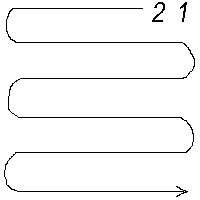
\includegraphics[scale=0.5]{example} \\
Примеры \\
(matrix-tr-br 4) => \\
\#2A((4  3   2  1) \\
    (5  6   7  8) \\
    (12 11 10  9) \\
    (13 14 15 16)) \\
	
}

\section{Оборудование студента}
{\large Процессор Intel(R) Core(TM) i5-8250U CPU @ 1.60GHz, память: 8192Gb, разрядность системы: 64.}

\section{Программное обеспечение}
{\large ОС Ubuntu 20.04 LTS, среда LispWorks Personal Edition 7.1.2}

\section{Идея, метод, алгоритм}
{\large 
Идея алгоритма простая. Функции {\tt matrix-tr-br (n)}, на вход подаётся порядок
матрицы. В этой функции создаём локальный двумерный массив. Затем циклом от 0 до n
проходимся по всем строкам (на n+1-ой итерации возращаем получившийся массив). 
Основная идея в том, что если мы находимся на строке с 
нечётным номером (строки номеруются с нуля), то будем заполнять строку слева направо
в возрастающем порядке. Первый элемент в нечётной строке будет равен {\tt n*i + 1} ({\tt i - } номер строки), т.к.
элемент над ним имеет значени {\tt n*i}. В чётной строке мы также идём слева направо, 
но элементы уже убывают. Следуя такому алгоритму, получим массив необходимого вида.
}

\section{Сценарий выполнения работы}

\section{Распечатка программы и её результаты}

\subsection{Исходный код}
\lstinputlisting{./lab3.lisp}

\subsection{Результаты работы}
% \lstinputlisting{./log2.lisp}

{\large 
	Для более удобной читаемости результата, результат функции {\tt matrix-tr-br}
	будем передовать в {\tt print-matrix}. (Функция взята со \href{http://lisp.ystok.ru/fp/help.html}{страницы курса.} )

CL-USER 12 > (print-matrix (matrix-tr-br 1)) \\

\#2A((1)) \\

CL-USER 13 > (print-matrix (matrix-tr-br 2)) \\

\#2A((2 1) \\
	(3 4)) \\

CL-USER 14 > (print-matrix (matrix-tr-br 3)) \\

\#2A((3 2 1) \\
    (4 5 6) \\
    (9 8 7)) \\

CL-USER 15 > (print-matrix (matrix-tr-br 4)) \\

\#2A((4 3 2 1) \\
    (5 6 7 8) \\
    (12 11 10 9) \\
    (13 14 15 16)) \\

CL-USER 16 > (print-matrix (matrix-tr-br 8)) \\

\#2A((8 7 6 5 4 3 2 1) \\
    (9 10 11 12 13 14 15 16) \\
    (24 23 22 21 20 19 18 17) \\
    (25 26 27 28 29 30 31 32) \\
    (40 39 38 37 36 35 34 33) \\
    (41 42 43 44 45 46 47 48) \\
    (56 55 54 53 52 51 50 49) \\
    (57 58 59 60 61 62 63 64)) \\
}

\section{Дневник отладки}
\begin{tabular}{|c|c|c|c|}
\hline
Дата & Событие & Действие по исправлению & Примечание \\
\hline
\end{tabular}

\section{Замечания автора по существу работы}
{\large 
Программа работает за $O(n^2)$. Так как мы проходимся по всей матрице.
}

\section{Выводы}
{\large 
В ходе выполнения лабораторной работы я познакомился с массивами. Узнал 
как с ними удобно работать и какие в нём есть преимущества, например массив знает свой размер.
Также получил опыт работы с циклами. Их отличительная черта от циклов, с которыми
я привык работать в императивных языках, в том, что они обязательно возращают значение.
\end{document}
